\chapter{楽曲制作}
\section{NoteSequenceの作成}
NoteSequenceとはMIDIデータから作成されるプロトコルバッファである.プロトコルバッファとは
NoteSequenceの作成は図のコマンドで作成できる.
\begin{figure}[!ht]
    \begin{screen}
    \begin{center}
        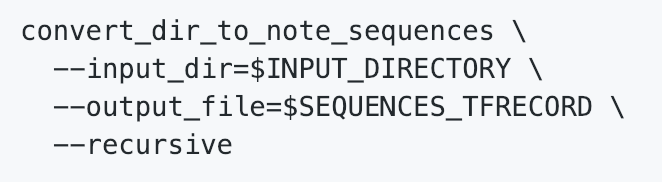
\includegraphics[scale=0.7, clip]{./img/Notesequence_make.png}
        \caption{NoteSequenceの作成}
        \label{fig:NoteSequenceの作成}
    \end{center}
    \end{screen}
    \end{figure}
\begin{itemize}
--inputdirで学習させるMIDIデータの 絶対パスを指定し,--outputfileでNotesequenceの出力先のディレクトリを指定する.\\
次に作成したNoteSequenceのデータセットを学習用と評価用に分割するために,下記のコマンドを実行する.
\begin{figure}[!ht]
    \begin{screen}
    \begin{center}
        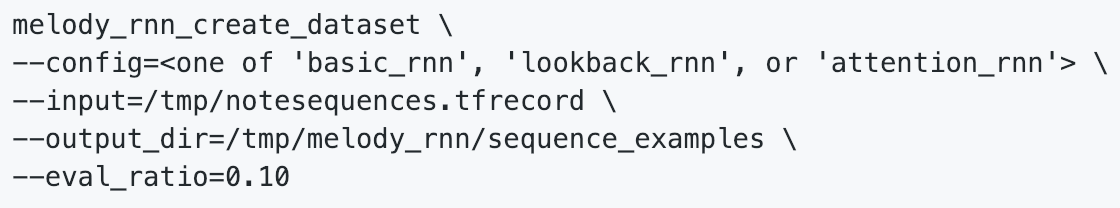
\includegraphics[scale=0.7, clip]{./img/Notesequence_split.png}
        \caption{NoteSequenceを学習用と評価表に分割}
        \label{fig:NoteSequenceを学習用と評価表に分割}
    \end{center}
    \end{screen}
    \end{figure}
\begin{itemize}
\subsection{BasicRNN}
\subsection{LookbackRNN}
\subsection{AttisionRNN}
\section{PolyfonyRNN}
